\section{Unavoidable Hazards of Bureaucracy\label{sec:unavoidable_hazards}}

In a bureaucracy there are certain challenges that cannot be avoided. The value of recognizing them is to understand that what you're experiencing isn't an anomaly. The problem isn't unique to you, your circumstances, your coworkers, or the organization. The cause is the combination of all those factors.

\ \\

\textbf{Separation of responsibility and accountability}. \\
Each bureaucrat in an organization has responsibilities associated with their role. The ability to complete the tasks associated the role are not wholly within the scope of the bureaucrat's control. Even if there is a desire for action, the action might not be immediately feasible because of a dependence on another person or process. 

\ \\

\textbf{Appreciation for being an effective bureaucrat is rare.}\\
If you do your job well, at best no one will notice.

``No one [thanks teachers] for policing cheating. Not the cheaters, not the honest students who feel inconvenienced and mistrusted, and certainly not the school [administrators] who have to process academic dishonesty paperwork.''\footnote{https://dynomight.net/teaching/}

The number of thank you cards sent to \href{https://www.fda.gov/}{Food and Drug Administration} meat inspectors, \href{https://www.osha.gov/}{Occupational Safety and Health Administration} regulators, \href{https://www.fcc.gov/}{Federal Communications Commission}, \href{https://www.ftc.gov/}{Federal Trade Commission}, and \href{https://www.sec.gov/}{Securities and Exchange Commission} is likely small. 
% TODO: ask each agency how many thank you letters they receive

There are counter examples in public service bureaucracy. 
Law enforcement is thanked when there is a victim of a crime. The military is held in high regard. 

\ \\

\textbf{Lack of accountability to fellow bureaucrats who rely on you.}\\
You are more likely to feel accountable to your supervisor. Performing for your supervisor and explaining your value matters more than the work done to support coworkers.  This also applies when you depend on other people -- they aren't accountable to you.

\ \\

\textbf{Decision-makers are under-informed and inexperienced.}\\
You can make a decision with insufficient information, and there is rarely an expectation of expertise or experience. 
Gathering information takes time and is thus burdensome.
Having experience requires getting experience.

\ \\

\textbf{Gathering data for decisions takes resources and expertise.}\\
When there is a desire to gather data, and there is data available to be gathered, an investment of time is necessary. Well-informed decisions take time, experience, or both.

\ \\

\textbf{Defining success is subjective and dynamic}. \\
Who defines success and for which audience in a bureaucratic organization is subjective because of the lack of feedback mechanisms. Consequences may not be immediately obvious. Worse, how success is defined can be changed at any time -- there's no need for consistency. 

\ \\

\textbf{Change threatens incumbents}. \\
Change of plans, roles, tasks, resources, flatness of org, scope, technology.

\ \\

\textbf{\href{https://en.wikipedia.org/wiki/Diffusion_of_responsibility}{Diffusion of responsibility} in the bureaucracy} \\
A specific task needs to be completed, and action requires involvement of multiple collaborators. 

Once responsibility is assigned, the new risk is that of blame.

\ \\

\textbf{Diffusion of blame in the bureaucracy}. \\
Example: if something goes wrong, who is at fault: the creator of a policy or the person tasked with executing the policy?

\ \\

\textbf{High latency feedback}. \\
See \S\ref{sec:slow_deployment} slow deployment of processes and \S\ref{sec:decision-delay} on decision delay.

\ \\

\textbf{Weak feedback}. \\
Suppose my bureaucratic task depends on a service provided by you, a fellow bureaucrat. If your computer isn't working, your ability to provide the service is blocked by a dependency on a computer repair person. You might feel relieved -- you can relax while you wait on the computer repair and you don't have to do work providing the service to me. You might feel anxious -- you're unable to provide the service until the computer is fixed. Regardless of how you feel about the situation, my task is blocked. If neither you nor I have priority relative to the computer repair person's other tasks, then we wait. This question of priority could be resolved hierarchically (for which there is limited attention bandwidth) or socially (dependent on someone having a relationship with the repair person). 

The delay for my task may be sufficiently small that raising the issue through the hierarchy or socially is not a good use of time.

\ \\

\textbf{The person making the rules that you follow doesn't actually know what they're doing}. \\
Your choices then include
\begin{itemize}
    \item Follow the rules that are not correct. This harms your productivity and morale. 
\item You can violate the rules and be more effective. This puts you at risk for sanctions. 
\item You can work the change the rules. Then you are not doing the work that's needed.
\end{itemize}


\ \\

\textbf{You rarely get to pick who is on the team}. \\
When a task requires collaboration, there is rarely a choice of who you get to work with. 

\ \\

\textbf{Rarely able to alter team membership.}

\ \\

\textbf{Fear of the unknown.}\\
Current suffering is tolerable compared to the uncertainty of change, especially when the suffering isn't felt by the decision maker.

By identifying this fear in yourself or those you collaborate with, you can discuss specific concerns and work to address them.
\marginpar{[Tag] Actionable Advice} 

\ \\

\textbf{Fear of change.} \\
Change disrupts the status quo, putting accumulated power at risk and altering relationships. 

An emotional basis for decision making (or avoidance of decision making) may or may not be rational. Discussing the fear with fellow bureaucrats can ease the burden. 

\ \\

\textbf{Fear of conflict.} Refers to conflict of ideas, not physical conflict. Conflict of ideas is not personal, though the consequences may have impacts on careers for stakeholders. \\
Professional disagreement is to be expected in a bureaucratic organization.

Feeling uncomfortable is distinct from feeling unsafe. Communicating while feeling discomfort is a useful skill, rather than avoidance. You can demonstrate courage by talking about your sense of discomfort. 

\ \\

\textbf{Inadequate resources: staffing, time, money.}\\
The resources you have to address a challenge may not match the complexity of the issue.

\ \\

\textbf{Outcomes for the team are ill-defined and constantly shifting.}\\

\ \\

\textbf{The reward for good work is more work.}\\
When a coworker doesn't do their fair share, then the productive employee shoulders more burden. The deficient worker has no incentive to improve

\ \\

\textbf{The organization has a lack of vision; or has vision but no plan; or has vision and a plan but no consensus; or has vision and a plan and consensus but inadequate resources.}

\ \\

\textbf{Progress depends on subjective decision making.}\\
Rarely is the optimal path deterministic. 

\ \\

\textbf{Easier to ask for big money than small money}\\
Processes are scale invariant -- Regardless of whether you're asking for \$1000 or \$100,000, the process is the same. 

\ \\

\textbf{Flux of people and processes.} \\
staff turn-over, changing conditions, changing timelines, change of vision, and the need to be promoted. in a bureaucracy, consistency doesn't yield promotion.

\ \\

\textbf{Why are there so many rules?}\\
To address edge cases and malicious or dumb people.

\ \\

\textbf{So much paperwork/forms.}
Why is Red tape endemic to bureaucracy?\\
Paperwork as a form of coordination in processes to facilitate decentralized decision making. 

One of the motives for paperwork is to catch people who are misrepresenting. Documentation makes prosecution more straightforward.

\ \\

\textbf{Everything is slower.}\\
What is meant is "slower than desired" or "slower than I imagined in my simplified model"

One reason progress is slower than expected is because there aren't as many hours available as imagined.


% What's the point of this? Is there a consequence for the reader?

In a bureaucracy the actual time spent working is less than the number of hours you get paid for. Breaks during work, vacation from work, holidays, sick leave. 

% https://rescuetime.wpengine.com/work-life-balance-study-2019/

\begin{figure}[H]
    \centering
    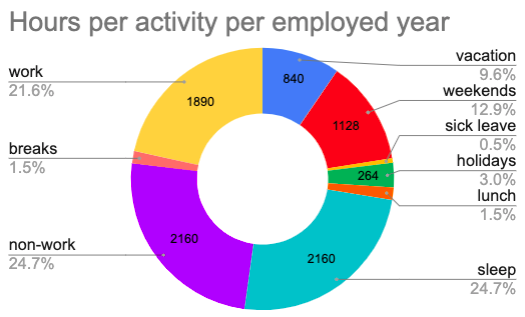
\includegraphics[width=0.8\textwidth]{images/hours_per_activity_per_employed_year}
    \caption{Hours of ``work'' per year when accounting for the rest of life. Assumes 5 weeks of vacation, 2 days of sick leave, and 11 holidays.}
    % footnotes in caption is not recommended; see https://texfaq.org/FAQ-ftncapt
    % however it can be done; see https://stackoverflow.com/questions/67621322/footnote-in-caption-of-figure-on-latex
    \label{fig:hours_per_year}
\end{figure}

Fig~\ref{fig:hours_per_year}
\footnote{\href{https://docs.google.com/spreadsheets/d/1ZaOZZXWkEzX4fFltUdlR4A6ENrAXnkzTW4YrjA4tDO8/edit?usp=sharing}{source for calculations}}

\ \\

\textbf{Bureaucracy inhibits creativity.}\\
See \S\ref{sec:innovation} for notes on innovation.

\ \\

% https://graphthinking.blogspot.com/2017/06/measuring-growth-of-bureaucracy.html
\textbf{Bureaucracy grows.}\\
The causes of growth include
scope creep, an increased number of people participating in the process, an increased workload, or the ratio of workers to managers decreases. 

You can measure the growth of bureaucracy using metrics like the latency in addressing a request and 
the number of people involved in addressing a request.  

\textbf{Increasing the size of a bureaucracy is easier than cutting it down.}\\
\ \\

% https://graphthinking.blogspot.com/2017/04/growth-of-bureaucracy.html
\textbf{The larger a hierarchy, the ratio of workers to managers gets worse}. \\

As complexity and workload increase, the number of staff needed increase. To facilitate coordination, managers arise. The amount of work being done in a bureaucracy can be small compared to the number of participants.

In Fig.~\ref{fig:growth_of_bureaucracy}a, the ratio of workers to participants is 3:3=1. When a manager is added, the ratio is 3:4 = 0.75 (a lower value means less work per employee is being accomplished). Adding a second team with dedicated management puts the ratio at 6:9=0.66. Finally, with a dedicated administrative team (e.g., payroll, hiring, facilities), the ratio is 6:13=0.46.

Adding more people to a hierarchical organization results in diminishing returns for time spent on the central work since bureaucrats invest time maintaining the hierarchy and administrative processes.

    \begin{figure}
        \centering
        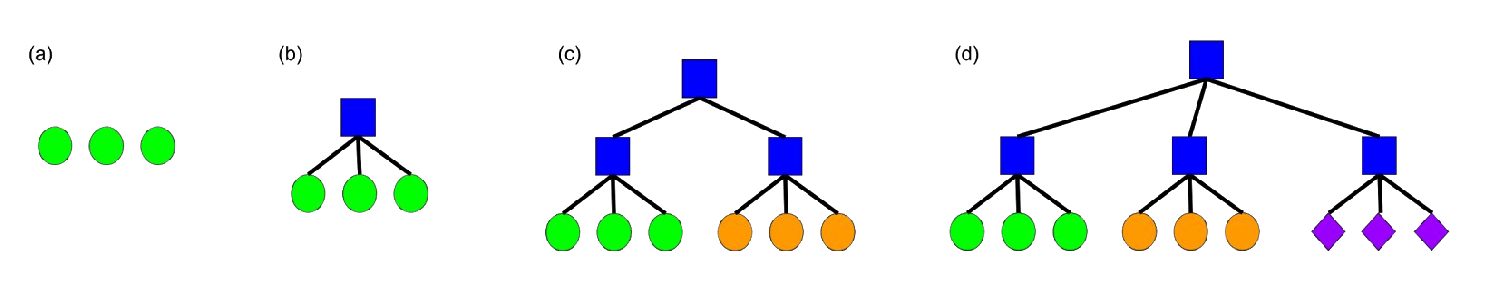
\includegraphics[width=1\textwidth]{images/growth-of-bureaucracy.pdf}
        \caption{Growth of an organization as complexity and workload increase. a: three technical workers (green dots); b: administrative functions are delegated to a administrative assistant or manager (blue square); c: as complexity and scale grows, a new technical team (orange dots) is brought in which has their own manager; d: administrative work is delegated to a dedicated team of non-technical staff (purple diamonds).}
        \label{fig:growth_of_bureaucracy}
    \end{figure}

\ \\

\textbf{Each person in a bureaucracy has multiple roles}.\\
To limit the expansion of the bureaucracy. The multiple roles come from multiple relationships necessary to span an organization larger than \href{https://en.wikipedia.org/wiki/Dunbar\%27s_number}{Dunbar's number}. 
\ \\

\textbf{Everything is more complicated}. \\
Bureaucracy administers access to resources, whether tangible items (water, air) or expertise. There's friction for tangible resources because the easiest solution is you get the resource (without an intermediary). There's friction for expertise because the expert understands things you do not. 

\ \\

\textbf{Bureaucracy is inefficient and wasteful.}\\
The inefficiency of an organization is not just due to a breakdown of communication among its many members. Different individuals in different roles faced distinct incentives and have a different view of what problem is most relevant. There is a mixture of competition and cooperation internally for resources.


Can you explain a Pareto frontier for multiple objectives like speed, cost, accuracy?

Because decisions by bureaucrats are subjective, there is significant risk of being wrong or being called out by others as being wrong. Therefore, a motive to cover your ass for decisions made. Unnecessary work is carried out. 

Different participants have different motives, and the aggregation needed for coordination is inefficient regardless of what metric efficiency is measured against.

Another example: Inefficiency of changing the requirements on a project partway through. If an objective quantitative measure were available, the return on investment could be determined. 

Efficiency is typically assessed from the perspective of a serial process -- a single worker could accomplish this task faster, so why involve 10 people and get a slower, more burdensome result? The Mythical Man Month manifests \href{https://en.wikipedia.org/wiki/Amdahl\%27s_law}{Amdahl's law}. Dividing a task among 10 people does not make the task 10x quicker. It's not valid to expect that a task which takes 1 person 1 hour to perfectly scale so 10 people should be able to accomplish 10 results in 1 hour.

Inefficiency of process is similar. I need to file a request to replace the lightbulb in my office. Compared to the serial ``I'll just replace the lightbulb myself by running to the hardware store and purchasing one."

The excess resources characterized as waste are similarly driven by the serial-based assessment of what one person would require to carry out the task. 

\ \\

% https://graphthinking.blogspot.com/2020/07/scope-creep-is-experienced-differently.html
\textbf{Scope creep.} \\
The customer wants more, and the exploration of what's possible is exciting (a positive experience).

The creator hears more work. This implies a few trade-off options, all of which are negative for one or both parties.
\begin{itemize}
    \item sticking with the original terms (telling the customer "no", which is negative for both parties)
    \item re-negotiation for additional compensation (a burden to both parties)
    \item the programmer doing more for the same pay, which means less money per effort (yielding a less happy programmer)
    \item decreasing existing efforts to fit the additional new requirements (yielding a less happy customer)
    \item even if the programmer is getting paid by the hour, additional work means the end product will be delayed to accommodate additional features (yielding a less happy customer)
\end{itemize}

\ \\

% https://graphthinking.blogspot.com/2020/09/why-migrating-from-current-to-new.html
\textbf{Migrating technologies.} \\
The person implementing the transition has to be educated in both the old and new technology. 
the legacy code has to be migrated to the new implementation
convincing stakeholders; may require synchronization
difficulty scales with the number of stakeholders 